\section{Software Development Process}
\label{sec:SoftwareDevelopmentProcess}

\subsection{Overview} 
The process of developing software is an extensive and complex process that requires a lot of planning, both in relation to the methodologies used during the development process and the requirements, both functional and non-functional of the software. This section details life cycle models considered for NeuraViz's development, the model that was eventually chosen, and modifications to the model necessary for the development of this particular system. It also lays out functional and non-functional requirements for NeuraViz.

\subsection{Life Cycle Model}
Prior to beginning development of NeuraViz, a number of software life cycle models were considered to govern the pace and structure of development. In all the waterfall model, iterative model, and agile model were considered. More specifically with agile, a variation of scrum, modified for a single developer, was considered. Ultimately, the modified scrum model was chosen for its flexibility and ability to adapt quickly to changing requirements.

\subsubsection{Waterfall Model}
The waterfall model is one of the oldest software development lifecycle (SDLC) models, originally proposed by Winston Royce in 1970 \cite{Gagan2020}. The model is a linear, sequential approach to software development, with each phase of the development process directly following the previous phase. Each subsequent phase relies on the previous phase, and as such the model does not allow going back to previous phases once they are completed. The first phase of the waterfall model is the requirement analysis phase, in which project requirements, both functional and non-functional, are gathered and documented. At this phase, requirements are also often analyzed for traits like consistency and feasibility. The second phase is the system design phase, in which the architecture of the software system is designed in full. All details of what needs to be done and how it will be completed are considered and documented during this phase. Third, the implementation phase is where the code for the software is written and the design from the previous step is implemented in full, exactly as specified during the design phase. During the fourth phase, the software is tested for bugs and errors, and issues are resolved as needed. Fifth, the software is deployed to the client in its entirety. In the waterfall model, this is the first time the client has seen the software. Finally, the software is maintained and updated as needed for as long as the client needs it. Figure \ref{fig:waterfall_model} shows a diagram of the waterfall model and its constituent parts.

Because of its rigid structure, the waterfall model excels at being very easy to understand and pick up quickly for new developers. In addition, it is easy to manage with relatively little overhead in management. When project requirements are well understood up front and unlikely to change, the waterfall model also serves the benefit of ensuring design is completed before implementation begins, which leads to fewer mistakes and less necessity to change the code once it has been written. However, for projects where requirements are less well understood or are likely to change, the waterfall model struggles to adapt and may lead to a design that was flawed in the first place with no way to fix it. In addition, the waterfall model does not allow for client feedback until the software is fully completed, which can lead to a lot of wasted time and effort if the client is not satisfied with the final product. 

\begin{figure}[htb]
    \centering
    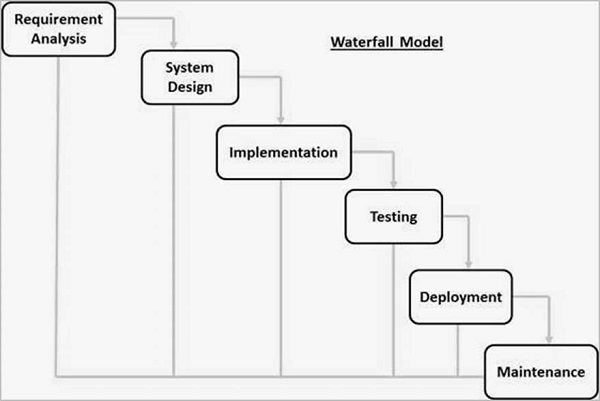
\includegraphics[width=.75\textwidth]{02_dev_process/res/sdlc_waterfall_model.jpg}
    \caption[Waterfall Model Diagram]{Waterfall Model Diagram \cite{tutorialspointWaterfall}}
    \label{fig:waterfall_model}
\end{figure}

\subsubsection{Iterative Model}
Like the waterfall model, the iterative model is mostly linear and sequential with a relatively rigid structure where each step directly follows the previous step. The phases in the iterative model as shown in Figure \ref{fig:iterative_model} roughly match those in the waterfall model, including a requirements analysis phase, a design phase, and implementation phase, a testing phase, and a deployment phase. Unlike the waterfall model, however, the iterative model runs these phases, with the exception of requirements analysis, multiple times, restarting the sequence of phases after each deployment. This serves the major benefit of allowing the ability for the client to give feedback on the project sooner and more often.

Due to its similarity to the waterfall model, the iterative model exhibits many of the same benefits of waterfall in that it is easy to understand with a relatively linear structure and minimal overhead. Like the waterfall model, when requirements are understood at the project outset, the design is likely to be almost fully complete before development begins, so the code is also less likely to require changes later in the process. While the iterative model does improve on the waterfall model's lack of ability for client feedback, it still struggles with changing requirements as each iteration of the project is still long and expected to be a relatively complete implementation of the software. The lack of adaptability made the iterative model a poor choice for NeuraViz's development where changing requirements were expected from the beginning.

\begin{figure}[htb]
    \centering
    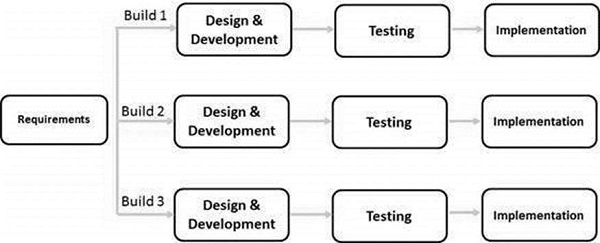
\includegraphics[width=0.75\textwidth]{02_dev_process/res/sdlc_iterative_model.jpg}
    \caption[Iterative Model Diagram]{Iterative Model Diagram \cite{tutorialspointIterative}}
    \label{fig:iterative_model}
\end{figure}

\subsubsection{Agile (Scrum) Model}
In contrast to the other models, agile models, and specifically scrum, was designed with the express intent to adapt to changing requirements quickly. Since the exact requirements and design for NeuraViz were not known well ahead of time, scrum was chosen for development due to its ability to pivot quickly when new design details were discovered. While agile is a category of software development models that focus on adaptability, scrum is a specific type of agile model that places emphasis on small, self-organized teams working in short, iterative cycles called sprints. Each sprint is typically two to four weeks long and ends with a review of the work completed during the sprint and a planning session for the next sprint. The scrum model is shown in Figure \ref{fig:scrum_model}. While the diagram shows a two to three month timeline per iteration, scrum more typically follows a shorter sprint length.

Since NeuraViz only has one developer, the scrum model doesn't fit perfectly. However, many aspects of the model do fit relatively well, with some slight modifications. Scrum typically emphasizes daily stand-up meetings with each team of developers. Due to the longer timeline of NeuraViz's development and the single developer, these meetings were partially dealt with through daily review of the project board to help ensure that projects stay on track. In addition, the developer met with the project advisor, Dr. Jason Sauppe, who in some sense served as a stakeholder on the project and a product owner. While these meetings don't match exactly with any part of the scrum model, they serve as a combination of stand-up meetings and sprint retrospectives. For the purposes of this project, sprints were completed every week. This allowed for very quick turnaround on features, and enabled constant feedback and reflection on project requirements.

% TODO: Maybe include burndown charts or something here?

\begin{figure}[htb]
    \centering
    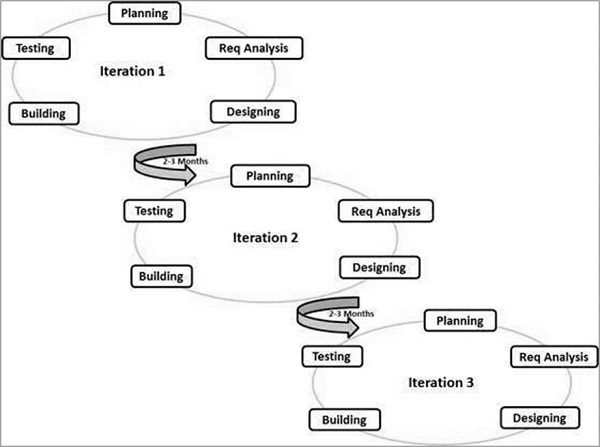
\includegraphics[width=0.75\textwidth]{02_dev_process/res/sdlc_agile_model.jpg}
    \caption[Scrum Model Diagram]{Scrum Model Diagram \cite{tutorialspointAgile}}
    \label{fig:scrum_model}
\end{figure}

\subsection{Functional Requirements}
Since agile methodologies were chosen for the development of this project, a set of functional requirements in the form of user stories were collected prior to the start of development. These user stories served as a guide for features to implement and helped ensure that no major functionality was missed during development.

NeuraViz is a relatively simple application with only one type of user. As such, the functional requirements are relatively straightforward, including the ability to upload a pre-trained machine learning model trained in either Pytorch or Keras. In addition, users should be able to see either the full graph of the uploaded model, or a collapsed version depending on the scale of the uploaded model. Additional functionality is also documented such as the ability to navigate the page via pan and zoom functionality on the graph, and clicking or hovering on various network components. 

In addition to the functionality of viewing the network itself, user stories were also documented for export functionality, allowing the graph of the model to be exported both as an svg and as a LaTeX document in the format of the tikz library. 

The full set of user stories is documented in \href{https://github.com/Bennett-Wendorf/NeuraViz/blob/main/docs/user_stories.md}{the user stories document}. This document also includes user stories for functionality that was not implemented in the current version of NeuraViz, but may be implemented in future versions.

\subsection{Non-Functional Requirements}
In addition to the functionality documented as user stories, non-functional requirements were also documented to ensure that the user experience of NeuraViz was as smooth as possible. Identified non-functional requirements are as follows:
\begin{itemize}
    \item Large network layers are collapsed if they are too big to reasonably render.
    \item If I am unable to view the model visually, labels exist for screen readers as much as possible.
    \item If the site takes a long time to load, skeletonized components are shown to indicate that the site is still loading.
    \item As a user, my data is reasonably secure, both during transmission and processing.
    \item Themes are sufficiently differentiable for colorblind users.
    \item Invalid models are rejected and not stored unnecessarily.
\end{itemize}
